\chapter{Основные сценарии использования системы}

\section*{Сценарии}

\subsection*{1. Поиск свободной аудитории}
\textbf{Предусловие:} Пользователь открыл телеграмм-бот.

\begin{enumerate}
    \item Пользователь вводит параметры поиска (например, время, вместимость
аудитории, наличие проектора).
    \item Система обращается к базе данных и ищет соответствующие свободные
аудитории.
    \item Система выводит пользователю список подходящих аудиторий.
    \item Пользователь может выбрать конкретную аудиторию для просмотра более
подробной информации.
\end{enumerate}

\subsection*{2. Просмотр расписания аудитории}
\textbf{Предусловие:} Пользователь находится в интерфейсе телеграмм-бота.

\begin{enumerate}
    \item Пользователь выбирает интересующую его аудиторию.
    \item Система извлекает и выводит текущее расписание для выбранной
аудитории.
\end{enumerate}

\subsection*{3. Автоматическое обновление информации о аудиториях}
\textbf{Предусловие:} На сайте home.mephi появилась обновленная информация о
кабинетах.

\begin{enumerate}
    \item По заданному расписанию или триггеру парсер начинает процесс
обновления данных.
    \item Парсер собирает актуальную информацию с сайта home.mephi.
    \item Обновленные данные записываются в базу данных.
    \item Если в процессе возникли ошибки, система отправляет уведомления
системному администратору.
\end{enumerate}

\chapter{Диаграммы последовательностей}

Поиск свободных кабинетов:
\begin{figure}[h]
    \centering
    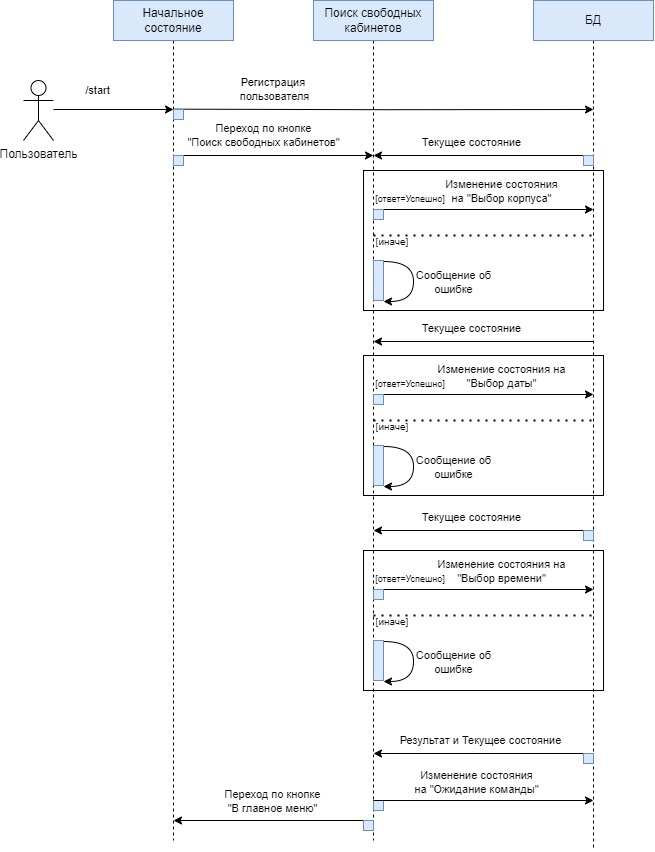
\includegraphics[scale=0.6]{img/seq1}
    \caption{диаграмма последовательности}
    \label{fig:cp}
\end{figure}

Получение информации о кабинете:
\begin{figure}[h]
    \centering
    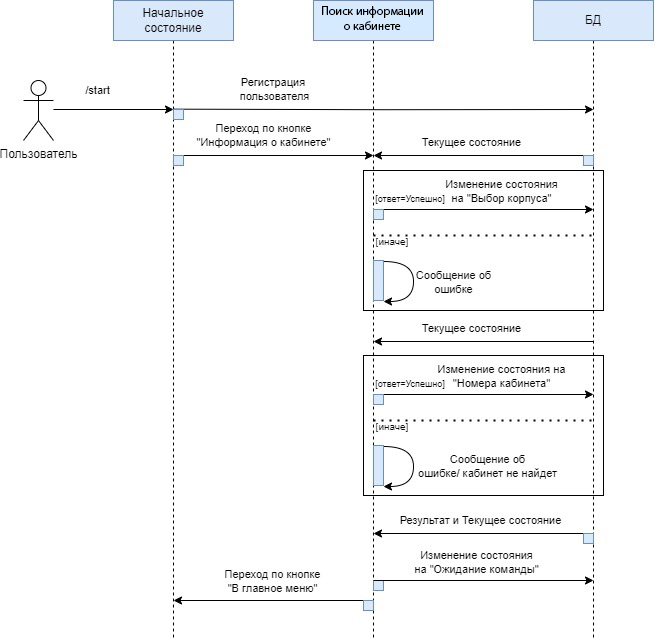
\includegraphics[scale=0.6]{img/seq2}
    \caption{диаграмма последовательности}
    \label{fig:cp}
\end{figure}